\textbf{Single Responsibility Principle}



    \textbf{Open/Closed Principle}
    
A relevant manifestation of \gls{ocp} are all the different implementations of expander
handlers in figure \ref{fig_handlers}. The availability of the
\code{koks_iexpanderhandlerinteractor_2023} interface makes it possible to add more
functionality to the CleanArchtictureExpander without modifying any existing
implementation. New handlers are added by extension, and when implemented correctly, the
handler is automatically executed in the desired order and the required conditions.

\lstinputlisting[
    caption={The \citetitle{koks_iexpanderhandlerinteractor_2023}},
    label={list_iexpanderhandlerinteractor} ]
    {Snippets/IExpanderHandlerInteractor.cs}

\lstinputlisting[
    caption={The \citetitle{koks_iexecutioninteractor_2023}},
    label={list_iexecutioninteractor} ]
    {Snippets/IExecutionInteractor.cs}

The fact that \citecode{koks_iexpanderhandlerinteractor_2023} derives from
\citecode{koks_iexecutioninteractor_2023} is another manifestation of \gls{ocp}. This
design decision allows for object types that need to be treated as executables by the
\code{koks_codegeneratorinteractor_2023}. Examples are
\citecode{koks_regionharvesterinteractor_2023},
\citecode{koks_regionrejuvenatorinteractor_2023},
\citecode{koks_preprocessorinteractor_2023} and
\citecode{koks_postprocessorinteractor_2023}. 

Listing \ref{list_CodeGeneratorInteractor} shows the
\code{koks_codegeneratorinteractor_2023} that cohesively executes all of the
\code{koks_iexecutioninteractor_2023} in order. The software engineer only has to focus on
implementing the specific type of \code{koks_iexecutioninteractor_2023} without having to
affect the implementation. This is by definition an example of \enquote{open for
extension} and \enquote{closed for modifications}.



\textbf{Interface segregation principle}
Take a look at Listing \ref{list_ispexample}. In order to comply with the \gls{isp}, the
design decision was made to separate all \gls{crud} operations into separate interfaces.
In the example of the \citecode{koks_appseederinteractor_2023} (see \ref{list_ispexample})
only the delete and create gateways where required. An alternative approach was to create
an IGateway interface containing all of the \gls{crud} operations. Following this approach
would lead to dependencies to all \gls{crud} operations in the
\code{koks_appseederinteractor_2023}.

\lstinputlisting[
    caption={The Gateways for Create, Read, Update, Delete operations},
    label={list_ispexample}]
    {Snippets/ISP_Example.cs}

    \textbf{dependency inversion principle}
    
Manifestations in the artifacts are ample. One of which is the consistent use of the
Dependency Injection pattern. In order to prevent the risks of displacing and dispersing
dependencies all over the system \parencite[214]{mannaert_normalized_2016} we are using
dependency containers. Each module is maintaining its own dependencies, which are
bootstrapped at application startup (see Listing \ref{list_dip})
\parencite{koks_generator_2023}.

\lstinputlisting[
    caption={Bootstrapping the dependencies of each component/layer of the
    generator artifact.},
    label={list_dip}]
    {Snippets/Dip.cs}

A more abstract example is the separation of required modules into separate component
libraries. This applies to both the generated and generator artifact (see Figure
\ref{fig_solutions}). The actual compliance to the \gls{dip} is how the flow of control
between the components is organized. This is accurately depicted in Figure
\ref{fig_modulair_components} \nameref{fig_modulair_components}.

\begin{figure}[H]
    \centering
    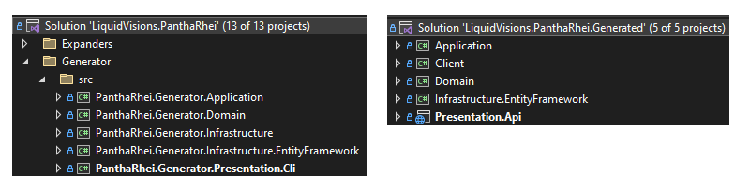
\includegraphics[width=1\textwidth]{figures/solutions.pdf}
    \caption[Separation of component libraries]{Separation of component libraries.}
    \label{fig_solutions}
\end{figure}